\documentclass[12pt]{article}
\usepackage{amsmath}
\usepackage{parskip}
\usepackage{gensymb}
\usepackage{graphicx}
\usepackage[letterpaper, margin=1in]{geometry}
\usepackage{fancyhdr}
\fancypagestyle{prelabheader} {
    \rhead{Raeed Hassan \\ hassam41}
    \lhead{\huge{ELECENG 2CI5 Lab 9 Prelab}}
}
\graphicspath{{./images/}}

\begin{document}
\newgeometry{margin=1in, includehead, head=47pt}
\thispagestyle{prelabheader}
i.\\
The frequency at which the average real power delivered to the load is maximized in a series RLC circuit is the resonance frequency, $f = \tfrac{\omega}{2\pi} = \tfrac{\tfrac{1}{\sqrt{LC}}}{2\pi}$. For the given circuit, the resonance frequency is $f = \tfrac{\tfrac{1}{\sqrt{LC}}}{2\pi} = \tfrac{\tfrac{1}{\sqrt{1\times10^{-3}\cdot1\times10^{-6}}}}{2\pi} = 5032.9$ Hz.

ii.
\begin{center}
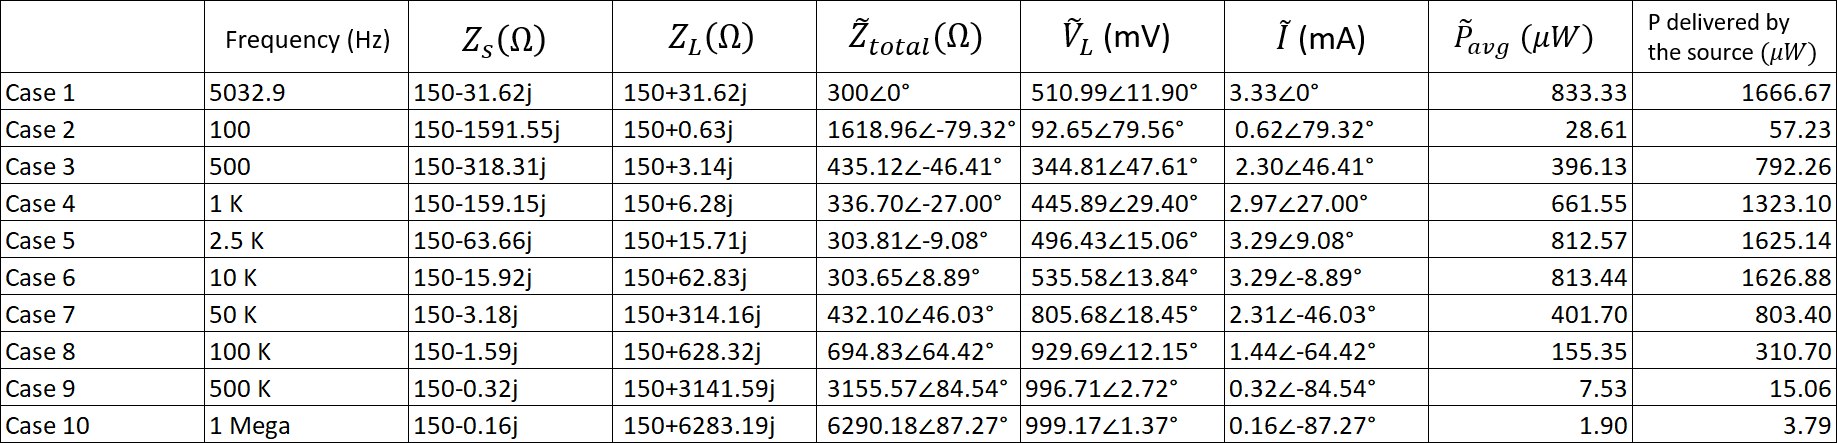
\includegraphics[width=\textwidth]{q2.png}
\end{center}
iii.

\begin{tabular}{|l|l|l|l|} 
    \hline
    & Frequency (Hz) & Calculated Phase Difference (\degree) & Measured Phase Difference (\degree) \\ \hline
    Case 1 & 5032.9 & 0 & 1.4 \\ \hline
    Case 2 & 100 & 79.32 & 75.5 \\ \hline
    Case 3 & 500 & 46.41 & 38.1 \\ \hline
    Case 4 & 1 K & 27.00 & 20.8 \\ \hline
    Case 5 & 2.5 K & 9.08 & 7.2 \\ \hline
    Case 6 & 10 K & -8.89 & -6.0 \\ \hline
    Case 7 & 50 K & -46.03 & -35.7 \\ \hline
    Case 8 & 100 K & -64.42 & -56.1 \\ \hline
    Case 9 & 500 K & -84.54 & -83.5 \\ \hline
    Case 10 & 1 Mega & -87.27 & -87.9 \\ \hline
\end{tabular}

The measured phase difference values were relatively similar to the calculated phase difference values, and followed the same pattern when frequency was changed.
\restoregeometry
\clearpage
iv.

\begin{tabular}{|l|l|l|}
    \hline
    & Frequency (Hz) & Measured Maximum Power (mW) \\ \hline 
    Case 1 & 5032.9 & 4.02 \\ \hline
    Case 2 & 100 & 0.59 \\ \hline
    Case 3 & 500 & 2.61 \\ \hline
    Case 4 & 1 K & 3.32 \\ \hline
    Case 5 & 2.5 K & 3.72 \\ \hline
    Case 6 & 10 K & 3.82 \\ \hline
    Case 7 & 50 K & 2.85 \\ \hline
    Case 8 & 100 K & 1.70 \\ \hline
    Case 9 & 500 K & 0.26 \\ \hline
    Case 10 & 1 Mega & 0.08 \\ \hline
\end{tabular}

\end{document}